\chapter{Classification with Fundamental Models}

In this chapter, we introduce \emph{reduced} and \emph{fundamental models} to classify discrete statistical models with rational MLE; this classification is due to Bik and Marigliano \cite{bik2022classifying}. 

\section{Parametrization}

First, we establish a parametrization for discrete statistical models with rational MLE, which is crucial for the classification of statistical models.

\begin{proposition}\label{prop:parametrization}
    Let \( \mathcal{M} \) be a one-dimensional discrete statistical models with rational MLE. Then, there exists a map of the form \( p: [0,1] \to \Delta_n, \theta \mapsto (w_k \theta^{i_k} (1-\theta)^{j_k})_{k=0}^n \) with \( i_k, j_k \in \mathbb{Z}_{\geq 0} \), \( w_k \in \mathbb{R}_{> 0} \) such that \( \mathcal{M} = \mathrm{image}(p) \).
\end{proposition}

We introduce some notation to simplify the proof of Proposition \ref{prop:parametrization}.
Let \( \mathcal{M} \subset \Delta_n \) be a one-dimensional discrete statistical model parametrized by rational functions \( p_0 =  \frac{g_0}{h_0}, \dots, p_n =  \frac{g_n}{h_n} \). Define \( b \coloneqq \mathrm{lcm}(h_0, \dots, h_n) \) and \( a_i \coloneqq b p_i \). Then, we multiply \( \sum_{k=0}^n p_k = 1 \) by \( b \) to obtain \( \sum_{k=0}^n a_k = b \). We use these polynomials \( a_0, \dots, a_n \) and \( b \) to determine the statistical model \( \mathcal{M} \). The log-likelihood function then reads
\begin{align*}
    \ell(p) = \sum_{k=0}^n u_k \log p_k = \sum_{k=0}^n u_k \log \frac{a_k}{b} = \sum_{k=0}^n u_k \log a_k - \sum_{k=0}^n u_k \log b.
\end{align*}
To find the maximum likelihood estimator, we find all critical points of the log-likelihood function, which is equivalent to finding the critical points of
\begin{align}\label{eq:score-equations}
    \ell(p(\theta))' &= \sum_{k=0}^n u_k \frac{a_k'}{a_k} - \sum_{k=0}^n u_k \frac{b'}{b} = 0.
\end{align}
These equations are called the \emph{score equations} in algebraic statistics.

\begin{definition}
    The number of complex solutions to the score equations for general data \( u \in \mathbb{C}^{n + 1} \) is called the \emph{maximum likelihood degree} (ML degree) of the statistical model. 
\end{definition}


This ML degree has an important meaning in algebraic statistics, as it is an algebraic measure of the complexity of the maximum likelihood estimation of the model \cite{amendola2019maximum, catanese2006maximum, sullivant2023algebraic}. We have the following relationship between MLE and ML degree.

\begin{proposition}\label{prop:rational-mle}
    A statistical model has rational maximum likelihood estimator if and only if the maximum likelihood degree of the model is one.
\end{proposition}

\begin{proof}
   Refer to \cite{duarte2021discrete} for a proof.
\end{proof}

Next, we need the following lemma to prove Proposition \ref{prop:parametrization},

\begin{lemma}\label{lem:two-complex-factors}
    Let \( \mathcal{M} \) be a one-dimensional discrete statistical models with rational MLE. Then, there exist exactly two distinct complex linear factors in \( a_0, \dots, a_n \), and \( b \).
\end{lemma}

\begin{proof}
    We prove the lemma in three steps:
    \begin{itemize}
        \item Let \( f \) be the product of all distinct complex linear factors in \( a_0, \dots, a_n\), and \( b \).  First, we multiply the score equations \eqref{eq:score-equations} by \( f \) to get \( f  \ell(p(\theta))' = \sum_{k=0}^n u_k f \frac{a_k'}{a_k} - \sum_{k=0}^n u_k f \frac{b'}{b} = 0 \).
        Note that every linear factor of \( a_k \) with multiplicity \( m \) occurs in \( a_k' \) with multiplicity \( m-1 \). Thus, \( \frac{a_k'}{a_k} = \frac{\lambda}{(x-\xi)} \) holds, where \( \lambda \in \mathbb{R} \) and \( x-\xi \) is some linear factor of \( a_k \). Hence, \( f \cdot  \frac{\lambda}{(x-\xi)}  \) is of degree \( \mathrm{deg}(f) - 1\). Therefore, \( f \ell(p(\theta))' \) is of degree \( \mathrm{deg}(f) - 1\).

        \item We claim that the roots of \( \ell(p(\theta))' \) are the same as the roots of \( f  \ell(p(\theta))' \). Assume that we have established this claim.  By Proposition \ref{prop:rational-mle}, the ML degree is one. So, \( \ell(p(\theta))' \) has one root. Thus, \( f  \ell(p(\theta))' \) has one root. Therefore, \( f  \ell(p(\theta))' \) is of degree one. This implies that \( \mathrm{deg}(f) = 2 \). Thus, there are exactly two distinct complex linear factors in \( a_0, \dots, a_n \), and \( b \).
        
        \item It remains to show that the roots of \( \ell(p(\theta))' \) are the same as the roots of \( f  \ell(p(\theta))' \). Clearly, every root of \( \ell(p(\theta))' \) is a root of \( f  \ell(p(\theta))' \). Conversely, we want to show that no new roots are introduced when multiplying by \( f \), i.e. roots of \( f \) are not roots of \(  f \cdot \ell(p(\theta))' \). Let us rewrite \( f  \ell(p(\theta))' = \sum_{k=0}^n u_k f \frac{a_k'}{a_k} - \sum_{k=0}^n u_k f \frac{b'}{b} = \sum_{k=0}^{n + 1} v_k f \frac{c_k'}{c_k} \)
        with \( v_k \coloneqq u_k, c_k \coloneqq a_k  \) for \( k=0, \dots,n \), and \(  v_{n+1} \coloneqq - \sum_{k=0}^n u_k \), \( c_{n+1} \coloneqq b \).

        Let \( q \) be a complex linear factor of \( f \). We define polynomials \( r_0, \dots, r_{n+1} \) and \( r \) such that \( c_k = q^{l_k}r_k \), \( f = q r \) hold, and \( r_0, \dots, r_{n+1}, r \) do not have \( q \) as a factor. Then, we have
        \begin{align*}
            f \frac{c_k'}{c_k} = q r \cdot \frac{l_k q^{l_k - 1} q'r_k +  q^{l_k}r_k'}{q^{l_k}r_k} = q r\frac{l_k q' }{q} + q r\frac{r_k'}{r_k} \equiv rl_k q' \pmod q
        \end{align*}
        for \(  k = 0, \dots, n+1 \).
        Thus, we obtain \( f \cdot \ell(p(\theta))' \equiv rq'\sum_{k=0}^{n + 1} v_k l_k \equiv rq' \sum_{k=0}^{n } v_k(l_k - l_{n+1}) \pmod q \).
        Note that by definition of \( l_k \), a value of \( l_k = 0 \) means that \( q \) is not a factor of \( c_k \). By definition of \( f \), at least one \( l_k \) is strictly positive. On the other hand, not all \( l_k \) can be strictly positive since \( a_0, \dots, a_n\), and \(b \) share no common factors. Hence, not all \( l_k - l_{n+1} \) vanish. Hence, for generic data \( u \) we assume \( \sum_{k=0}^{n } v_k(l_k - l_{n+1}) \neq 0 \). This with \( q'r \not \equiv 0 \pmod q \) implies that \( q \) is not a complex linear factor of \( f  \ell(p(\theta))' \). We showed that the roots of \( f \) are not roots of \( f \cdot \ell(p(\theta))' \).
    \end{itemize}
\end{proof}

We now prove Proposition \ref{prop:parametrization}.

\begin{proof}
    First, we show that \( I \) is a single closed real interval and not a union of closed intervals. For the sake of contradiction, assume that \( I = \bigcup_{k} I_k \) is a union of closed disjoint intervals. By definition of \( \mathcal{M} \), we know that \( p(\partial I) \subset \partial \Delta_n \). Thus, there exist \( \theta_1, \theta_2 \in \partial I_0 \) and \( \theta_3, \theta_4 \in \partial I_1 \) with \( p_i(\theta_1) = p_i(\theta_2) =  0 \) and \( p_j(\theta_3) = p_j(\theta_4) = 0 \) for some \( i,j = 0, \dots, n \). Note that \( \theta_1 \) and \( \theta_2 \) are roots of \( \frac{a_i}{b} \); similarly,  \( \theta_3 \) and \( \theta_4 \) are roots of \( \frac{a_j}{b} \). By Lemma \ref{lem:two-complex-factors}, exactly two distinct complex linear factors occur in \( a_0, \dots, a_n \), and \( b \). Hence, \( \theta_3 = \theta_1 \) or \( \theta_3 = \theta_2 \) holds. We found a contradiction for \( I_0 \) and \( I_1 \) are disjoint.

    We established that \( I = [\alpha, \beta ]\) is a real single closed interval. Thus, the roots of \( a_0, \dots, a_n\), and \( b \) are real and take values in \( \partial I = \left\{ \alpha, \beta \right\} \). By a suitable parametrization, we assume \( I = [0,1] \). Next, we write the polynomials \( a_0, \dots, a_n\), and \( b \) as \(  a_k(\theta) = w_k \theta^{i_k} (1-\theta)^{j_k} \) and \( b(\theta) = w \theta^{i} (1-\theta)^{j} \)
    with \( w_k, w \in \mathbb{R}_{>0} \), and \( i_k, j_k, i, j \in \mathbb{Z}_{\geq 0} \). Since \( a_0, \dots, a_n\), and \( b \) share no common factors, there exists some \( i_k = 0 \) if \( i > 0 \); however, this contradicts \(0 < w_k \leq a_0(0) + \dots + a_n(0) = b(0) = 0\). So, \( i = 0 \) holds. Similarly, we have \( j = 0 \). Finally, we divide \( p \) by \( w \) to obtain \( b \equiv 1 \).
\end{proof}

\begin{corollary}
    Any one-dimensional {discrete} {statistical} {models} with rational MLE can be represented by \( (w_k, i_k, j_k)_{k=0}^n \) for \( w_k \in \mathbb{R}_{>0} \) and \( i_k, j_k \in \mathbb{Z}_{\geq 0} \).
\end{corollary}

\begin{definition}
    The \emph{degree} \( \mathrm{deg}(\mathcal{M}) \) of a one-dimensional discrete statistical models with rational MLE \( \mathcal{M} \) represented by \( (w_k, i_k, j_k)_{k=0}^n \) is defined as \( \mathrm{max}\left\{ i_k + j_k : k = 0, \dots, n \right\} \).
\end{definition}

\begin{remark}\label{rem:equivalent-models}
    We view two models \( (w_k,i_k,j_k)_{k=0}^n \) and \( (w_k',i_k',j_k')_{k=0}^n \) as the same model if they are equal up to a permutation of the coordinates.
\end{remark}

\begin{example}
    The sequence \( ((1,0,2), (2,1,1), (1,2,0)) \) represents the binomial model with two trials. It has degree two. Its parametrization is given by \( \theta \mapsto ((1-\theta)^2, 2\theta(1-\theta),\theta^2) \). See Figure \ref{fig:binom-discrete-model} for a visualization of the binomial model within the probability simplex \( \Delta_2 \). Note that we treat \( ((1,0,2), (2,1,1), (1,2,0)) \), \( ((2,1,1), (1,0,2), (1,2,0)) \), and \( ((2,1,1), (1,2,0), (1,0,2)) \) as the same model, as coordinate order does not matter.
\end{example}

\begin{definition}
    Let \( \mathcal{M} \) be a model represented by \( (w_k, i_k, j_k)_{k=0}^n \). The set of exponent pairs \( (i_k, j_k)_{k=0}^n \) is called the support of \( \mathcal{M} \), denoted by \( \mathrm{supp}(\mathcal{M}) \).
\end{definition}

Throughout the remainder of this thesis, we adopt the convention that models refer to one-dimensional discrete statistical models with a rational MLE.


\section{Reduced Models}

The first building block for the classification of models are \emph{reduced models}.


\begin{definition}
    We call a model represented by \( (w_k, i_k, j_k)_{k=0}^n \) \emph{reduced} if \( (i_k, j_k) \neq \mathbf 0 \) for all \( k = 0, \dots, n \), and \( (i_k, j_k) \neq (i_l, j_l) \) for all \( k \neq l \).
\end{definition}

Next, we use functions to represent reduced models due to \( (i_k, j_k) \neq (i_l, j_l) \).

\begin{remark}\label{rem:representation-of-models-by-functions}
    A reduced model \( \mathcal{M} \) represented by \( (w_k, i_k, j_k)_{k=0}^n \) is identified by a function \( f: \mathbb{Z}^2 \to \mathbb{R}_{\geq 0}, (i, j) \mapsto w \), where \( w = w_k \) if \( (i_k, j_k) = (i, j) \) and \( w = 0 \) otherwise. The support of \( f \) is the set of all pairs \( (i, j) \) with \( f(i, j) > 0 \). It coincides with the support of \( \mathcal{M} \).
\end{remark}


Reduced models are our first building blocks for the classification of statistical models because the following two propositions show that non-reduced models are transformed into a reduced model by a sequence of linear embeddings.

\begin{proposition}\label{prop:linear-embedding-1}
    Let \( n \in \mathbb{N}_{>0} \) and \( \mathcal{M} \) be a statistical model represented by \( (w_k, i_k, j_k)_{k=0}^n \). If \( (i_l, j_l) = \mathbf{0} \) for some index \( l \in \mathbb{N} \), then there exist \( \mathcal{M}' \), \( \lambda \in [0,1] \) and \( k \in \{ 0, \dots, n \} \) such that \( \mathcal{M} = \Psi_{\lambda,k}(\mathcal{M}') \), where \( \Psi_{\lambda, k}: \Delta_{n-1} \to \Delta_n \) is defined as \(  p_i \mapsto \begin{cases}
        \lambda p_i & \text{if } k \neq i, \\
        1-\lambda & \text{otherwise}
    \end{cases} \).
\end{proposition}

\begin{proof}
    Let \( (i_l, j_l) = (0,0) \) for some index \( l \in \mathbb{N} \). If \( w_l = 1 \), then \( w_m = 0 \) for all \( m \neq l \); this contradicts \( w_m > 0 \) by Proposition \ref{prop:parametrization}. Set \( \lambda \coloneqq 1 - w_l > 0 \) and \( k \coloneqq l \). Define the statistical model \( \mathcal{M}' \) by \( \left(\frac{w_h}{1-w_l}, i_h, j_h\right)^n_{h=0, h \neq l} \).
    Then, \( \mathcal{M} = \Psi_{\lambda,k}(\mathcal{M}') \) holds.
\end{proof}

\begin{proposition}\label{prop:linear-embedding-2}
    Let \( n \in \mathbb{N}_{>0} \).
    Let \( \mathcal{M} \) be model represented by \( (w_k, i_k, j_k)_{k=0}^n \). If \( (i_m, j_m) = (i_l, j_l)  \) for \( m \neq l \), then there exist \( \mathcal{M}' \), \( \lambda \in [0,1] \) and \( k,h = 0, \dots, n \) such that \( \mathcal{M} = \Psi_{\lambda,k,h}(\mathcal{M}') \), 
    where we define \( \Psi_{\lambda, k,h}: \Delta_{n-1} \to \Delta_n,  p_i \mapsto \begin{cases}
         p_i & \text{if } i \notin \left\{ k,h \right\}, \\
        \lambda p_k & \text{if } k = i, \\
        (1-\lambda) p_k & \text{if } h = i. \\
    \end{cases} \)
\end{proposition}

\begin{proof}
    Set \( \lambda \coloneqq \frac{w_m}{w_m + w_l} \), \( k \coloneqq m \), and \( h \coloneqq l \). Define \( \mathcal{M}' \) by \(  \left( w_g + \delta_{gm}w_l, i_g, j_g  \right)^n_{g=0, g \neq l} \).
    Then, \( \mathcal{M} = \Psi_{\lambda,k}(\mathcal{M}') \) holds.
\end{proof}

Repeated application of these propositions transforms any model into a reduced model.

\begin{corollary}\label{cor:reduced-models}
    Let \( n \in \mathbb{N}_{> 0} \).
    If \( \Delta_n \) contains a model of degree \( d \), then there exists \( m \leq n \) such that \( \Delta_m \) contains a reduced model of degree \( d \).
\end{corollary}


\section{Fundamental Models}

We present \emph{fundamental models}, which are building blocks for reduced models.

\begin{definition}\label{def:fundamental-model}
    We call a model \( \mathcal{M} \) represented by \( (w_k, i_k, j_k)_{k=0}^n \) \emph{fundamental} if it is reduced and the equation \( \sum_{k=0}^n p_k  = \sum_{k=0}^n x_k \theta^{i_k} (1-\theta)^{j_k} = 1, \forall \theta \in [0,1] \) has a unique solution \( (x_k)_{k=0}^n \) with \( x_k = w_k \).
\end{definition}

\begin{example}
    Consider the binomial model with two trials. Its exponent pairs read \( (i_0, j_0) = (0,2) \), \( (i_1, j_1) = (1,1) \), and \( (i_2, j_2) = (2,0) \). Then, the equation is \( p_0 + p_1 + p_2 = x_0\theta^2 + x_1\theta(1-\theta) + x_2(1-\theta)^2 \equiv 1 \); it has a unique solution \( w_0 = 1, w_1 = 2, w_2 = 1 \). To see this, observe that the equation is equivalent to \( x_0\theta^2 + x_1\theta - x_1 \theta^2 + x_2 -2x_2\theta + x_2\theta^2 = 1\), which in turn is equivalent to solving \( x_2 - 1 + \theta(x_1 - 2x_2) + \theta^2(x_0 - x_1 + x_2) = 0 \) for all \( \theta \in [0,1] \). Thus, the binomial model is fundamental.
\end{example}

\begin{example}\label{ex:prob-simplex-0}
    The probability simplex \( \Delta_0 \) only contains the model \( 1 \), which is fundamental.
\end{example}

\begin{example}\label{ex:prob-simplex-1}
    Consider \( \Delta_1 \). It only contains the models \( \theta \mapsto (\theta, 1-\theta) \) and \( \theta \mapsto (1-\theta, \theta) \). Both models are equivalent and fundamental.
\end{example}

We use \emph{composition} to construct reduced models from fundamental models.

\begin{definition}
    Let \( \mu \in (0,1) \). Let \( \mathcal{M} \) and \( \mathcal{M}' \) be reduced models represented by \( f,g : \mathbb{Z}^2 \to \mathbb{R}_{\geq 0} \). The \emph{composite} \( \mathcal{M} *_\mu \mathcal{M}' \) is defined as the model represented by \(  (i,j) \mapsto \mu f(i,j) + (1-\mu) g(i,j) \). It is easy to see that \( \mathcal{M} *_\mu \mathcal{M}' \) is a reduced model.
\end{definition}



% \begin{proposition}
%     Let \( \mathcal{M} \) be a reduced model. If \( \mathcal{M} \) is not the composite of two reduced models whose supports are proper subsets of \( \mathrm{supp}(\mathcal{M}) \), then \( \mathcal{M} \) is fundamental.
% \end{proposition}

% \begin{proof}
%     Let \( S \coloneqq \mathrm{supp}(\mathcal{M}) \) and let \( \mathcal{M} \) be represented by \( (v_k, i_k, j_k)_{k=0}^n \). The set of all reduced models with support equal to \( S \) corresponds to the set \( A \) of all real \( (w_k)_{k=0}^n \) that satisfy 
%     \begin{align*}
%         \sum_{k=0}^n w_k t^{i_k}(1-t)^{j_k} \equiv 1, \quad w_k \in \mathbb{R}.
%     \end{align*}
%     This set \( A \) contains \( v \). It is an affine-linear half-space, and its dimension coincides with the dimension of the linear space  \( \mathrm{lin}\{ t^{i_k}(1-t)^{j_k} : k=0, \dots, n\} \) since there exists an open ball around \( \mathbf v \) containing only positive vectors.

%     By assumption \( \mathcal{M} \) is the composite of two reduced models \( \mathcal{M}_1 \) and \( \mathcal{M}_2 \) with supports \( S_1 \) and \( S_2 \) which are proper subsets of \( S \).
% \end{proof}

\begin{proposition}\label{prop:composition-fundamental}
    Every reduced model is the finite composite of fundamental models.
\end{proposition}

\begin{proof}
    The simplices \( \Delta_0 \) and \( \Delta_1 \) contain only fundamental models by Example \ref{ex:prob-simplex-0} and \ref{ex:prob-simplex-1}. 
    
    Assume \( n \geq 2 \). Let \( \mathcal{M} \in \Delta_n \) be a model that is not fundamental. We aim to show that \( \mathcal{M} \) can be expressed as a composite of two models, \( \mathcal{M}' \) and \( \mathcal{M}'' \), whose supports are proper subsets of \( \mathrm{supp}(\mathcal{M}) \). Assume this is indeed the case. Then, by applying the same argument to \( \mathcal{M}' \) and \( \mathcal{M}'' \), we can recursively decompose each non-fundamental model into models with smaller supports. Since \( \mathrm{supp}(\mathcal{M}) \) is finite, this recursive decomposition eventually terminates, yielding a decomposition of \( \mathcal{M} \) into fundamental models. Thus, we have shown that any reduced model is the composite of a finite number of fundamental models. 

    Let us prove that \( \mathcal{M} \) is the composite of two models whose supports are proper subsets of \( \mathrm{supp}(\mathcal{M}) \). Since \( \mathcal{M} \) is not fundamental, the equation \( p_0 + \dots + p_n = 1 \) has distinct solutions \( \mathbf w, \mathbf w' \in \mathbb{R}^{n+1}_{> 0} \). Define \( \mathbf v \coloneqq \mathbf w - \mathbf w' \neq \mathbf 0 \). Then, for all \( \theta \in (0,1) \) we have \( \sum_{k=0}^n v_k \theta^{i_k}(1-\theta)^{j_k} = 0  \).
    Observe that there are strictly positive and negative coefficients \( v_k \). 
    
    We define \( \lambda \coloneqq \min \left\{ \frac{w_k}{\lvert v_k \rvert} : k = 0, \dots, n, \; v_k < 0 \right\} \), \( u_k \coloneqq w_k + \lambda v_k \) for \(k = 0, \dots, n \), and \( S_1 \coloneqq \left\{ (i_k, j_k) : k=0, \dots, n, \; u_k \neq 0 \right\} \). Note that \( \lambda > 0 \) since all the coefficients \( w_k \) are strictly positive by definition. Also observe that \( u_k \geq 0 \) if \( v_k \geq 0 \). Moreover, we have \( \frac{w_k}{\lvert v_k \rvert} \geq \lambda \) for all \( k \geq 0 \). Hence, if \( v_k < 0 \) holds, we have \( \frac{u_k}{v_k} = \frac{w_k}{v_k} + \lambda  \leq 0\). Multiplying by \( v_k < 0 \), we obtain \( u_k \geq 0 \). All in all, we have \( u_k \geq 0 \) for all \( k = 0, \dots, n \). Moreover, \( u_k = 0 \) holds if and only if \( v_k < 0 \) and \( \lambda = \frac{w_k}{\lvert v_k \rvert} \) holds. This shows that \( S_1 \subsetneq \mathrm{supp}(\mathcal{M}) \). Since we have \( u_0 + \dots u_n = 1 \), we found a reduced model \( \mathcal{M}' \) represented by \( (u_k, i_k, j_k)_{(i_k,j_k) \in S_1} \).

    For the second model \( \mathcal{M}'' \), we define \( \mu \coloneqq \min \left\{ \frac{w_k}{u_k} : k = 0, \dots, n, \; u_k \neq 0 \right\} \), \( t_k \coloneqq \frac{w_k - \mu u_k}{1 - \mu} \) for \(  k = 0, \dots, n \), and \( S_2 \coloneqq \left\{ (i_k, j_k) : k=0, \dots, n, \; t_k \neq 0 \right\} \).
    As before, we have \( \mu > 0 \). Additionally, \( \mu < 1 \) holds because we have \( v_k > 0 \) implying \( u_k > w_k \). By definition, we have \( t_k \geq 0 \) and \( t_k = 0 \) if and only if \( u_k \neq 0 \) and \( \mu = \frac{w_k}{u_k} \). This shows that \( S_2 \subsetneq  \mathrm{supp}(\mathcal{M}) \) and \( S_1 \cup S_2 = \mathrm{supp}(\mathcal{M}) \). Since \( t_0 + \dots + t_n = 1 \), we found a reduced model \( \mathcal{M}'' \) represented by \( (t_k, i_k, j_k)_{(i_k,j_k) \in S_2} \).

    Finally, we see that \( w_k = \mu u_k + (1-\mu) t_k\). This shows that \( \mathcal{M} = \mathcal{M}' *_\mu \mathcal{M}'' \).
\end{proof}

Applying the previous proposition with Corollary \ref{cor:reduced-models} yields the following corollary.

\begin{corollary}\label{cor:fundamental-models-ksmlkdf}
    If \( \Delta_n \) contains a non-fundamental model of degree \( d \), then there exists a fundamental model of degree \( d \) in \( \Delta_m \) for some \( m < n \).
\end{corollary}

\begin{example}
We classify all models for \( \Delta_2 \). Note that the model \( \mathcal{M} \) parametrized by \( \theta \mapsto (\theta, 1-\theta) \) satisfies \( \mathcal{M} *_\mu \mathcal{M} = \mathcal{M} \) for all \( \mu \in (0,1) \). Since \( \Delta_1 \) only contains this model, we conclude that \( \Delta_2 \) only contains fundamental or non-reduced models.

To find all fundamental models in \( \Delta_2 \), we check for all sets \( S = \left\{ (i_k,j_k)\right\}_{k=0}^2 \subset \mathbb{Z}^2_{>0} \) of size three if the equation \( p_0 + p_1 + p_2 = 1 \) has a unique solution. A priori, infinitely many sets \( S \) must be checked; we will see in the next section that it suffices to check only those sets \( S \) with degree \( \mathrm{deg}(S) \coloneqq \max\left\{ i+j : (i,j) \in S \right\}  \) at most three. An exhaustive search yields the following supports for fundamental models: \( \{ (0,3), (1,1), (3,0) \}\), \( \{ (0,2), (1,1), (2,0) \}\), \( \{ (0,1), (1,1), (2,0) \} \), and \( \{ (0,2),(1,0),(1,1) \} \); they correspond to fundamental models \( ((1-\theta)^3, 3\theta(1-\theta), \theta^3) \), \( ((1-\theta)^2, 2\theta(1-\theta), \theta^2) \), \( (1-\theta, \theta(1-\theta), \theta^2) \), and \( ((1-\theta)^2, \theta, \theta(1-\theta)) \).  Note that the last model is viewed as equivalent to the third model because we can use the parametrization \( \theta \mapsto 1-\theta \) and a suitable permutation of the coordinates to obtain the third model.

\begin{figure}[H]
    \centering
    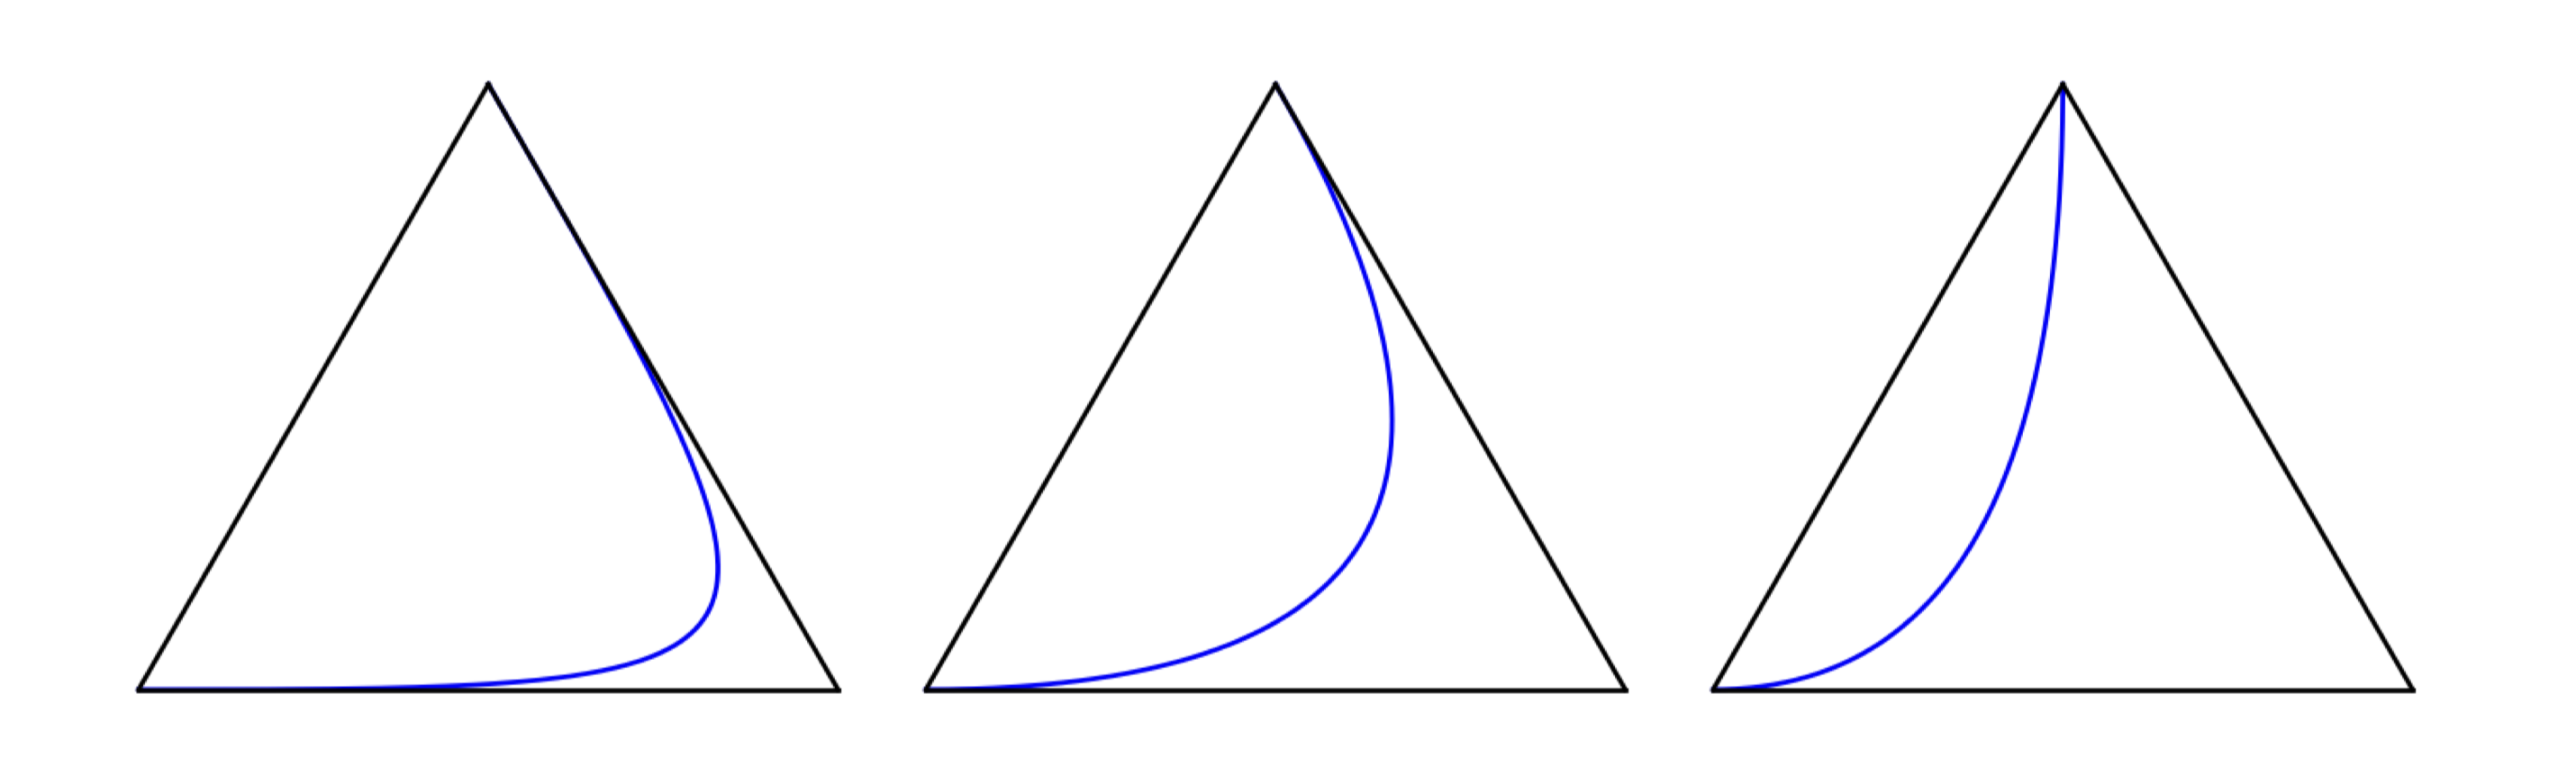
\includegraphics[width=0.9\textwidth]{assets/fundamental-models-delta-2.png}
    \caption{From left to right, the illustration depicts the models parametrized \( ((1-\theta)^3, 3\theta(1-\theta), \theta^3) \), \( ((1-\theta)^2, 2\theta(1-\theta), \theta^2) \), \( (1-\theta, \theta(1-\theta), \theta^2) \), and \( ((1-\theta)^2, \theta, \theta(1-\theta)) \).}
\end{figure}

We have computed all fundamental models of degree at most three in \( \Delta_2 \). Of course, there exist non-reduced models, too. They come from linear embeddings \( \Psi_{\lambda,k} \) and \( \Psi_{\lambda,k,h} \), and for \( \lambda = \frac{1}{3} \) we obtain the models \( \theta \mapsto (\frac{2}{3}\theta, \frac{1}{3}, \frac{2}{3}(1 - \theta)) \) and \( \theta \mapsto (1-\theta, \frac{1}{3}\theta, \frac{2}{3}\theta) \).

\begin{figure}[H]
    \centering
    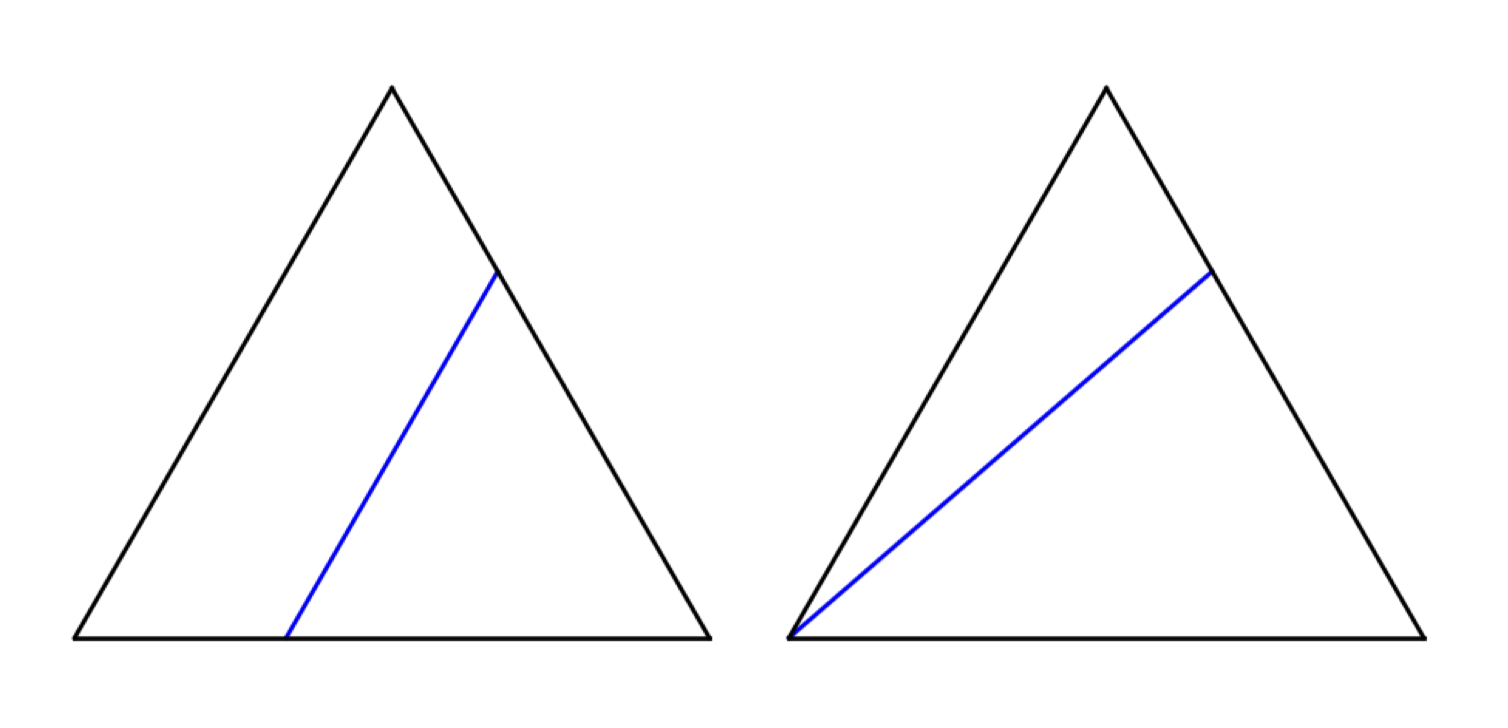
\includegraphics[width=0.66\textwidth]{assets/non-red-models-delta-2.png}
    \caption{This illustration depicts two non-reduced models in \( \Delta_2 \) parametrized by \( \theta \mapsto (\frac{2}{3}\theta, \frac{1}{3}, \frac{2}{3}(1 - \theta)) \) and \( \theta \mapsto (1-\theta, \frac{1}{3}\theta, \frac{2}{3}\theta) \).} 
\end{figure}
\end{example}

\begin{theorem}\label{thm:classification-jekns}
    Every model in \( \Delta_n \) is the image of a reduced model in \( \Delta_m \) under a linear embedding \( \Delta_m \to \Delta_n \) for some \( m \leq n \). Moreover, every reduced model \( \mathcal{M} \subset \Delta \) can be written as a composite of finitely many fundamental models \( \mathcal{M} = \mathcal{M}_1 *_{\mu_1} ( \dots *_{\mu_{m-2}}( \mathcal{M}_{m-1} *_{\mu_{m-1}} \mathcal{M}_m) ) \)
    for some \( m < n \) and \( \mu_1, \dots, \mu_m \in (0,1) \).
\end{theorem}

\begin{proof}
    See Proposition \ref{prop:composition-fundamental}, Proposition \ref{prop:linear-embedding-1}, and Proposition \ref{prop:linear-embedding-2}.
\end{proof}

\section{On the Finiteness of Fundamental Models}



After establishing that fundamental models are building blocks for all models, we dedicate ourselves to the proof that only finitely many fundamental models in \( \Delta_n \) for \( n \leq 4 \) exist -- a result that was first established by Bik and Marigliano \cite{bik2022classifying}.

\begin{theorem}\label{thm:degree-fundamental-models}
    Let \( \mathcal{M} \in \Delta_n \) be a model. For \(n \leq 4 \), we have \( \mathrm{deg}(\mathcal{M}) \leq 2n - 1\).
\end{theorem}

Given this theorem, it is easy to show the finiteness of fundamental models.

\begin{theorem}\label{thm:finiteness-fundamental-models}
    There are only finitely many fundamental models in \( \Delta_n \) for all \( n \leq 4 \).
\end{theorem}

\begin{proof}
    Let \( n \leq 4 \).
    By Theorem \ref{thm:degree-fundamental-models}, we know that the degree of a fundamental model is at most \( 2n - 1 \). Since the number of supports of a fundamental model of degree \( 2n - 1 \) is finite, there are only finitely many fundamental models in \( \Delta_n \).
\end{proof}

It turns out that proving Theorem \ref{thm:degree-fundamental-models} only for fundamental models is sufficient.

\begin{theorem}\label{thm:degree-fundamental-models-reduced}    
    Let \( N \in \mathbb{N} \). If the upper bound \( \mathrm{deg}(\mathcal{M}) \leq 2n - 1 \) holds for all \( n \leq N \) and for all fundamental models \( \mathcal{M} \in \Delta_n \), then this upper bound also holds for all statistical models, including non-fundamental ones, in \( \Delta_n \) for all \( n \leq N \).
\end{theorem}

\begin{proof}
    Let $N \in \mathbb{N}$ and $n \leq N$.
    Assume that there is a non-fundamental model $\mathcal{M}'$ in $\Delta_n$ of degree greater than $2n - 1$. By Corollary \ref{cor:fundamental-models-ksmlkdf}, there exists a fundamental model $\mathcal{M}$ in $\Delta_m$ of degree greater than $2m - 1$ for some $m < n$. This contradicts the assumption that the degree of fundamental models is at most $2k - 1$ for all $k \leq N$.
\end{proof}

This justifies that our north star is to prove the following theorem.

\begin{theorem}\label{thm:degree-fundamental-models-fundamental}
    Let \( \mathcal{M} \) be a fundamental model in \( \Delta_n \). For \(n \leq 4 \), we have \( \mathrm{deg}(\mathcal{M}) \leq 2n - 1\).
\end{theorem}

The first step towards our north star is introducing a combinatorial puzzle to count fundamental models using the defining sequence \((w_k, i_k, j_k)_{k=0}^{n}\).